\section{The CMS trigger system}
%%%%%%%%%%%%%%%%%%%%%%%%%%%%%%%%%%
\label{sec:Trigger}

The LHC can provide proton-proton interactions at a crossing frequency of 40\,MHz and, for each bunch crossing, several collisions can occur (approximately 20 at the nominal instantaneous luminosity). Since it is impossible to store and process the large amount of data associated with the resulting large number of events, a drastic rate reduction has to be achieved. In fact the speed at which data can be written to mass storage is limited and, moreover, the vast majority of events produced is not interesting for physics analyses, because it involves low transverse momentum interactions (also called \emph{minimum bias events}). The task of reducing this rate is accomplished by the CMS trigger system, which is the start of the physics event selection. CMS makes use of a two-stage trigger system, consisting of a \emph{Level-1} trigger (L1)~\cite{Dasu:2000ge} and a \emph{High Level Trigger} (HLT)~\cite{Cittolin:578006}.

Level-1 trigger runs on dedicated processors, and accesses coarse level granularity information from calorimetry and muon system. A L1 Trigger decision has to be taken for each bunch crossing within $3.2\,\mathrm{\mu s}$. Its task is to reduce the data flow from 40\,MHz to about 100\,kHz.

The High Level Trigger is responsible for reducing the L1 output rate down to a maximum rate of the order of 1\,kHz. The HLT code runs on a farm of commercial processors and can access the full granularity information of all the sub-detectors.

The main characteristics of the CMS trigger system are described in the following.

%%%%%%%%%%%%%%%%%%%%%%%%%%%%%%%%%%%%%%%%%%%%%%%%%%%%%%%%%
\subsection{The Level-1 trigger}

The L1 trigger is responsible for the identification of electrons, muons, photons, jets and missing transverse energy. It is required to have a high and carefully understood efficiency. Its output rate and speed are limited by the readout electronics and by the performances of the data
acquisition (DAQ) system~\cite{Cittolin:578006}. It consists of three main subsystems:
\begin{itemize}
\item L1 Calorimeter Trigger;
\item L1 Muon Trigger;
\item L1 Global Trigger.
\end{itemize}
The L1 Global Trigger is responsible for combining the output of L1 Calorimeter
Trigger and L1 Muon Trigger and for making the decision to either retain the event or discard it. The organization of CMS L1 Trigger is schematically summarized in Fig.~\ref{fig:trigL1}.
\begin{figure}[htb]
\centering
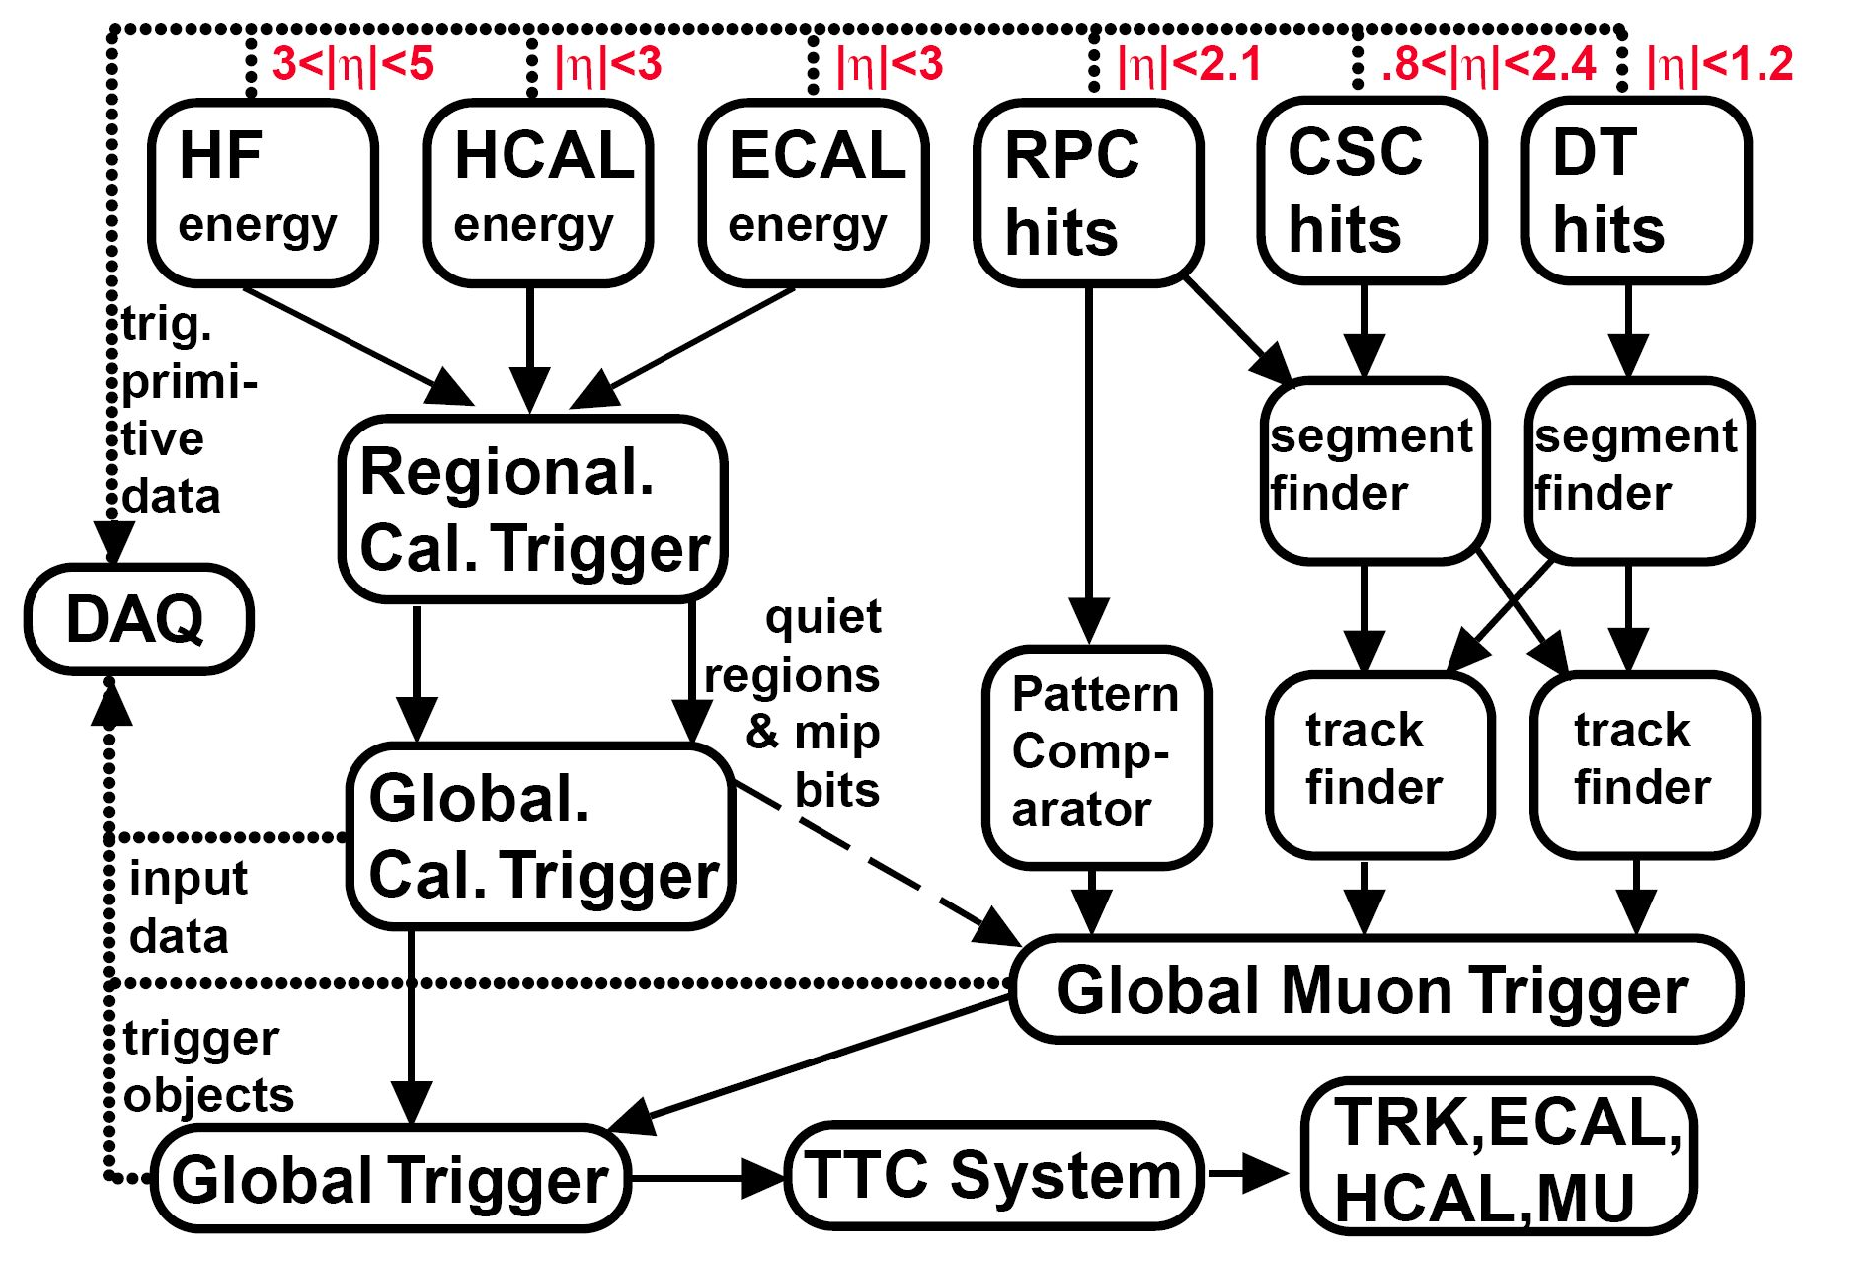
\includegraphics[width=0.7\textwidth]{images/trigL1.png}
\caption{Schematic representation of the Level-1 trigger components.}\label{fig:trigL1}
\end{figure}

\subsubsection{L1 Calorimeter Trigger}
\textcolor{red}{Controllare se è stato cambiato qualcosa nel Run2}

The input for the L1 Calorimeter Trigger are calorimeter towers, which are clusters of signals collected both from ECAL and HCAL. Towers are calculated by calorimeter high level readout circuits, called Trigger Primitive Generators. The Regional Calorimeter Trigger identifies electron, photon, $\tau$ and jet candidates together with their transverse energy and sends the information to the Global Calorimeter Trigger. The Global Calorimeter Trigger sorts the candidates according to their transverse energy and sends the first four objects to the L1 Global Trigger.

\subsubsection{L1 Muon Trigger}
\textcolor{red}{Controllare se è stato cambiato qualcosa nel Run2}

The L1 Muon Trigger is actually a composite system istelf: information from RPC, CSC and DT specific triggers are combined in the so called L1 Global Muon Trigger. 

The RPC trigger electronics builds Track Segments, gives an estimate of their \pt and sends these segments to the Global Muon Trigger. It also provides the CSC logic unit with information to solve hit position ambiguities in case of two or more muon tracks crossing the same CSC chamber. 

The CSC trigger builds Local Charged Tracks (LCT), that is track segments made out of the cathode strips only, and assign a \pt value and a quality falg to the LCTs. The best three LCTs in each sector of nine CSC chambers are passed to the CSC Track Finder, that uses the full CSC information to build tracks, assigns them a \pt and a quality flag and sends them to the Global Muon Trigger.

DTs are equipped with Track Identifier electronics, which is able to find groups of aligned hits in the four chambers of a superlayer. Those Track Segments are sent to the DT Track Correlator that tries to combine segments from two superlayers, measuring the $\phi$ angle. The best two segments are sent to the DT Track Finder that builds tracks and sends them to the Global Muon Trigger.

The Global Muon Trigger sorts the RPC, CSC and DT muon tracks and tries to combine them. The final set of muons is sorted according to the quality, and the best four tracks are passed to the L1 Global Trigger.

\subsubsection{L1 Global Trigger}
\textcolor{red}{Controllare se è stato cambiato qualcosa nel Run2}

The L1 Global Trigger is responsible for collecting objects created from the Calorimeter and Muon Triggers and for making a decision whether to retain the event or not. In case the event is accepted, the decision is sent to the Timing Trigger and Control System, that commands the readout of the remaining subsystems.

In order to take the decision, the L1 Global Trigger sorts the ranked objects produced by calorimetry and muon system and checks if at least one of the thresholds in the L1 trigger table is passed.

%%%%%%%%%%%%%%%%%%%%%%%%%%%%%%%%%%%%%%%%%%%%%%%%%%%%%%%%%
\subsection{The high level trigger (HLT)}

The High Level Trigger is designed to reduce the L1 output rate down to about 1000\,$\mathrm{events/s}$, which is the amount that will be written to mass storage. HLT code runs on commercial processors and performs reconstruction using the information from all sub-detectors. Events passing
the HLT are stored on local disk or in CMS Tier 0\footnote{The Worldwide LHC Computing Grid (WLCG) is composed of four levels, or ``Tiers'', identified with numbers 0, 1, 2 and 3. Each Tier is made up of several computer centres and provides a specific set of services; they process, store and analyse all the data from the Large Hadron Collider (LHC). Tier 0 is the CERN Data Centre. All of the data from the LHC pass through this central hub. Tier 0 distributes the raw data and the reconstructed output to Tier 1's, and reprocesses data when the LHC is not running.}. 

Data read from sub-detectors are assembled by a builder unit and then assigned to a switching network that dispatches events to the processor farm. The CMS switching network has a bandwidth of 1 Tbit/s. This simple design ensures maximum flexibility to the system, the only limitation being the total bandwidth and the number of processors. The system can be easily upgraded adding new processors or replacing the existing ones with faster ones as they become available. Since the algorithms have a fully software implementation, improvements to the algorithms can be easily implemented and do not require any hardware intervention.

Event by event, the HLT code is run on a single processor, and the time available to make a decision is about 300 ms. The real time nature of this selection imposes several constraints on the resources an algorithm can use. The reliability of HLT algorithms is of capital importance, because events not selected by the HLT are lost. In order to efficiently process events, the HLT code has to be able to quickly reject not interesting events; computationally expensive algorithms must be run only on good candidates for interesting events. In order to cope with this requirement the HLT code is organized
in a virtually layered structure:
\begin{itemize}
\item Level 2: uses only complete muon and calorimetry information;
\item Level 2.5: uses also the pixel information;
\item Level 3: makes use of the full information from all the tracking detectors.
\end{itemize}
Each step reduces the number of events to be processed in the following step. The most computationally expensive tasks are executed in the Level 3; time consuming algorithms such as track reconstruction are only executed in the region of interest. Besides, since the ultimate precision is not required at a HLT level, track reconstruction is performed on a limited set of hits, and is stopped once the required resolution is achieved.








